\subsection{Introduction}

\begin{frame}{RIOT}
\framesubtitle{Introduction}
\begin{columns}
\begin{column}{0.5\textwidth}
 \begin{itemize}
  \item Un OS pour l'IoT
  \begin{itemize}
    \item CAN
    \item BLE (NimBLE)
    \item LoRaWAN
    \item SigFox
    \item 6LoWPAN, Thread
  \end{itemize}
  \item Tickless scheduler
  \begin{itemize}
    \item Basse consommation
  \end{itemize}
  \item Temps reel
  \item API pour les drivers
  \item build, flash et console facile
  \begin{itemize}
    \item \lstinline{make flash term}
  \end{itemize}
\end{itemize}
\end{column}
\begin{column}{0.5\textwidth}
\makebox[\linewidth]{
\includegraphics[width=\textwidth]{presentation.tex/fig/riot.png}}
\end{column}
\end{columns}
\end{frame}

\begin{frame}{RIOT}
\framesubtitle{Introduction}
\begin{center}
\scalebox{0.45}{%
\begin{tikzpicture}
\path[mindmap,concept color=black,text=white]
  node[concept] {RIOT OS}
  [clockwise from=0]
  child[concept color=green!50!black] {
    node[concept] {OS}
    [clockwise from=90]
    child[concept color=green!60!black] { node[concept] {Driver} }
    child[concept color=green!60!black] { node[concept] {Thread} }
    child[concept color=green!60!black] { node[concept] {Concurence} }
    child[concept color=green!60!black] { node[concept] {Message} }
  }  
  child[concept color=blue] {
    node[concept] {IoT}
    [clockwise from=-30]
    child[concept color=blue!70] { node[concept] {LPWAN, Ethernet, WiFi} }
    child[concept color=blue!70] { node[concept] {CoAP, MQTT} }
    child[concept color=blue!70] { node[concept] {RPL} }
  }
  child[concept color=red] { 
    node[concept] {Compatibilité} 
    [clockwise from=-80]
    child[concept color=red!80]  { 
      node[concept] {Framework} 
      [clockwise from=-45]
      child[concept color=red!60] { node[concept] {Arduino} }
      child[concept color=red!60] { node[concept] {MicroPython} }
      child[concept color=red!60] { node[concept] {LUA} }
      child[concept color=red!60] { node[concept] {Jerryscript} }
    }
    child[concept color=red!80]  { 
      node[concept] {Lib} 
      [counterclockwise from=-140]
      child[concept color=red!60] { node[concept] {Tensorflow} }
      child[concept color=red!60] { node[concept] {SSL} }
    }
    child[concept color=red!80]  { 
      node[concept] {Language} 
      [counterclockwise from=-140]
      child[concept color=red!60] { node[concept] {C++} }
    }
  }
  child[concept color=orange] { 
    node[concept] {Autres} 
    [counterclockwise from=90]
    child[concept color=orange!80] { node[concept] {FATfs} }
    child[concept color=orange!80] { 
      node[concept] {100+ boards} 
      [counterclockwise from=120]
      child[concept color=orange!60] { node[concept] {ESP32} }
      child[concept color=orange!60] { node[concept] {STM32} }
      child[concept color=orange!60] { node[concept] {ATMEGA} }
      child[concept color=orange!60] { node[concept] {Native} }
    }
    child[concept color=orange!80] { node[concept] {Exemples} }
  };
\end{tikzpicture}
}
\end{center}

\end{frame}

\begin{frame}{RIOT}
\framesubtitle{Concurrence}
\begin{columns}
\begin{column}{0.6\textwidth}
 \begin{itemize}
  \item Une approche 'from scratch'
  \begin{itemize}
    \item Pas de dependance constructeur
    \item Driver maison
  \end{itemize}
  \item Communauté accessible
  \item Beaucoups de drivers
  \item Beaucoups de plateformes
  \begin{itemize}
    \item Support pour le low-end
    \item Support CPU 8, 16 bits
  \end{itemize}
\end{itemize}
\end{column}
\begin{column}{0.4\textwidth}
\begin{center}
  
\includegraphics[width=0.9\textwidth]{presentation.tex/fig/armmbed.png}
  
\includegraphics[width=0.8\textwidth]{presentation.tex/fig/zephyr.png}
\end{center}
\end{column}
\end{columns}
\end{frame}

\begin{frame}
\frametitle{RIOT}
\framesubtitle{Hardware}
\begin{columns}
  \begin{column}{0.35\textwidth}
  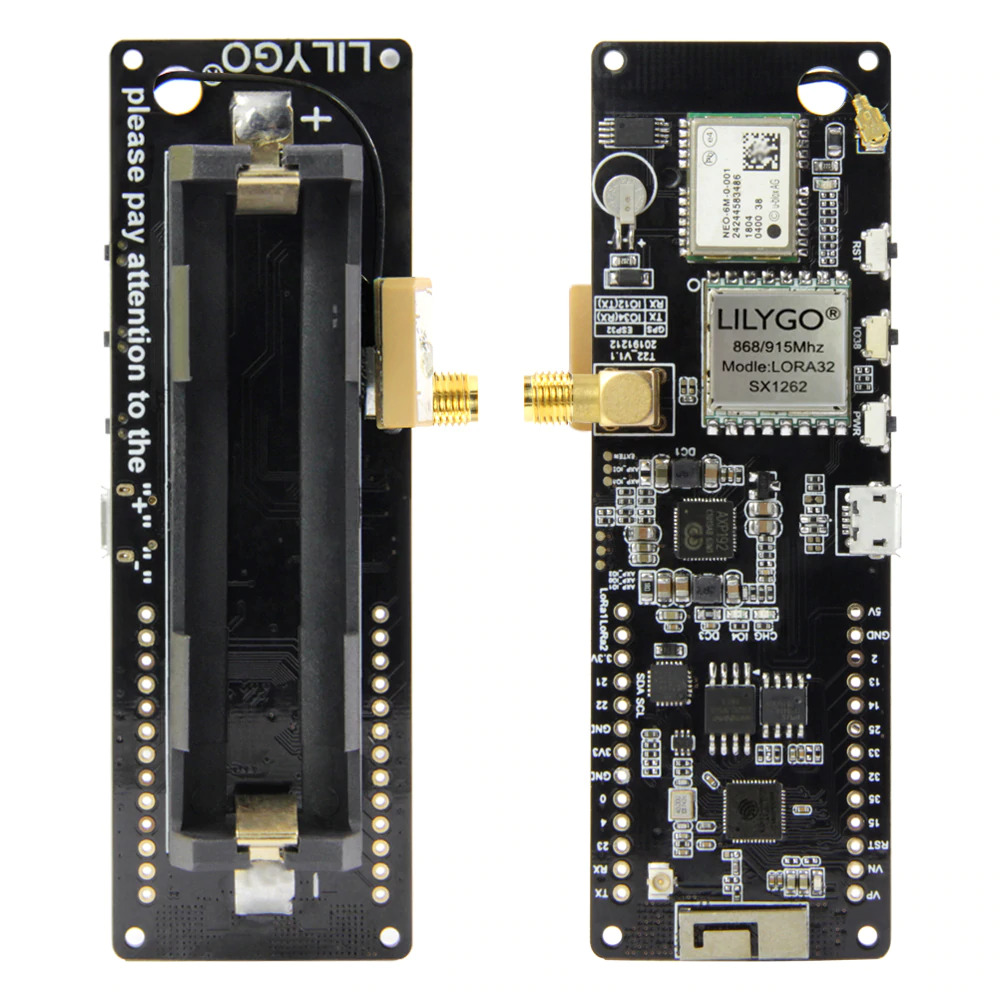
\includegraphics[width=0.9\textwidth]{presentation.tex/fig/loramote1.jpg}
  \end{column}
  \begin{column}{0.35\textwidth}
  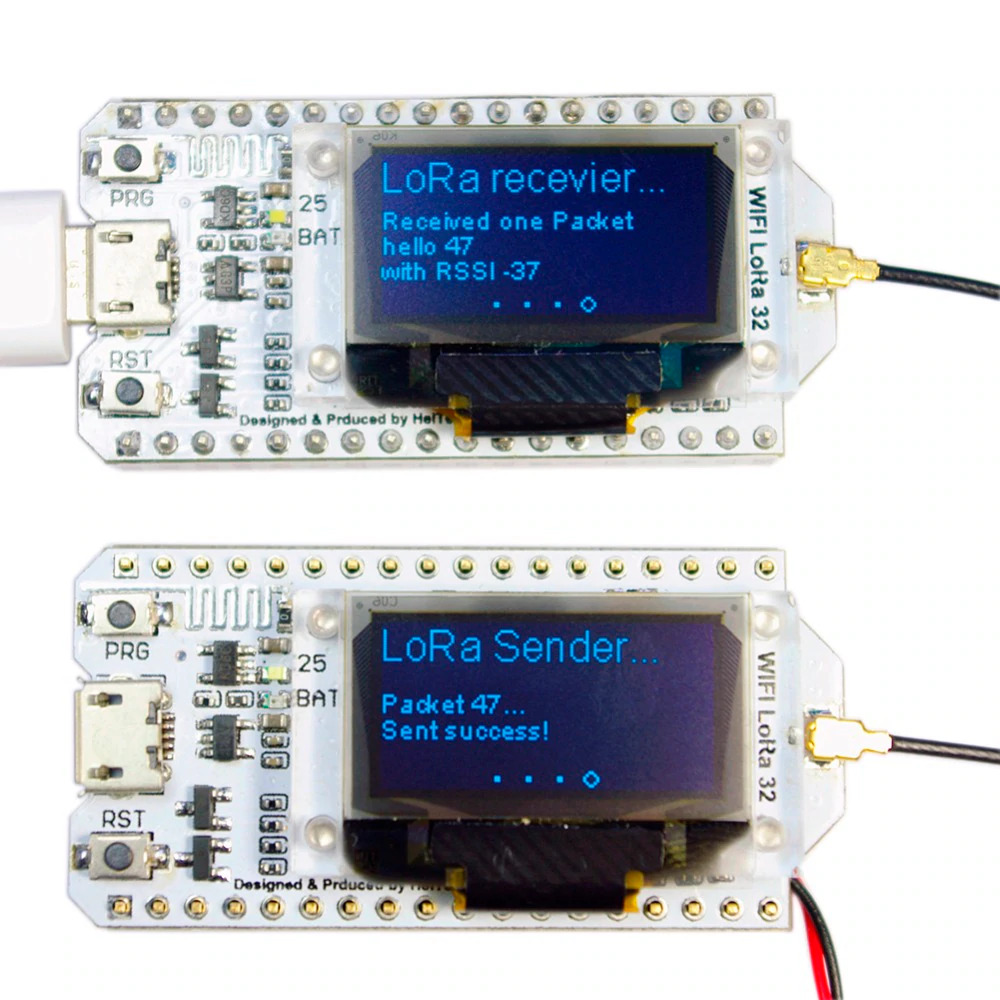
\includegraphics[width=0.9\textwidth]{presentation.tex/fig/loramote2.jpg}
  \end{column}
  \begin{column}{0.3\textwidth}
  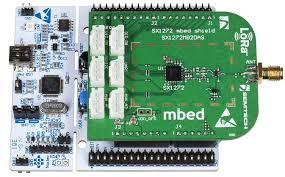
\includegraphics[width=0.9\textwidth]{presentation.tex/fig/loramote3.jpg}
  \end{column}
\end{columns}
  
\end{frame}

\subsection{Utilisation}

\begin{frame}[fragile]
\frametitle{RIOT}
\framesubtitle{Utilisation}
  
\begin{minted}{bash}
$ ls ./boards/
arduino-uno
arduino-zero
bluepill
calliope-mini
esp32-heltec-lora32-v2
esp32-mh-et-live-minikit
esp32-ttgo-t-beam
esp32-wemos-lolin-d32-pro
esp8266-esp-12x
esp8266-olimex-mod
native
nucleo-f030r8
stm32f0discovery
wemos-zero
\end{minted}

\end{frame}

\begin{frame}[fragile]
\frametitle{RIOT}
\framesubtitle{Utilisation}

\begin{minted}{bash}
$ make -C <example_dir> BOARD=<board_dir_name> flash
$ make -C <example_dir> BOARD=<board_dir_name> term
\end{minted}
  
\end{frame}

\begin{frame}
\frametitle{RIOT}
\framesubtitle{Utilisation}
\begin{itemize}
  \item Exemple
  \begin{itemize}
    \item \href{https://github.com/RIOT-OS/RIOT/tree/master/examples/gnrc_lorawan}{$examples/gnrc_lorawan$}
  \end{itemize}
  \item Cours
  \begin{itemize}
    \item \href{https://riot-os.github.io/riot-course/slides/02-getting-started/}{Getting started}
    \item \href{https://riot-os.github.io/riot-course/slides/03-riot-basics}{Riot basics}
  \end{itemize}
\end{itemize}
\end{frame}

